\section*{Algorithms for solving IVPU game}
To construct the whole diagram of $\omega(P)$ in $[0,P^*]$, we need to obtain the specific subsidy value $\omega(P)$ given any $P$, which is piecewise linear and convex at every sub-interval. As long as we find all breakpoints during the interval, to get the whole diagram we just need to connect these breakpoints in order.

At first, we need to divide the interval into $v$ sub-intervals according to the number of machines used by the grand coalition. However, we don't need to calculate the interval $[0,P_{\lceil v+1/2 \rceil}]$ because at this part the corresponding subsidy is 0 always.(The corresponding conclusion we mentioned in Theorem \ref{thm4})
Then we just need to apply the IPC algorithm on the rest interval to get the breakpoints. After obtaining all the breakpoints, the PSPF function can be constructed.


\begin{algorithm}[h]\label{algoIPC}
\caption{The Intersection Points Computation(IPC) Algorithm to Construct the PSPF Function.}
\begin{algorithmic}[1]

\begin{description}
  \justifying
  \item[Step 1.] Initially, set $I^*=\{P_L,P_H\}$ and $\mathbb{I}= \{[P_L,P_H]\}$.
  \item[Step 2.] If $\mathbb{I}$ is not empty, update $I^*$ and $\mathbb{I}$ by the following steps:
  \item[Step 3.] Sort values in $I^*$ by $P_0<P_1<\cdots<P_q$, where $P_0 = P_L,P_q = P_H$ and $q = |I^*|-1$.
  \item[Step 4.]
  Select any interval from $\mathbb{I}$, denoted by $[P_{k-1},P_{k}]$ with $1\leq k \leq q$
  \item[Step 5.]
  Construct two linear function $ R_{k-1}(P)$ and $ L_{k}(P)$ so that $ R_{k-1}(P)$ passes $(P_{k-1},\omega(P_{k-1}))$ with \\
  \vspace{10pt}
  a slope equal to a right derivative $K_{r}^{P_{k-1}}$ of $\omega(P)$ at $P_{k-1}$, and that $L_{k}(P)$ passes $(P_{k},\omega(P_{k}))$ with a \\
  \vspace{10pt}
  slope equal to a left derivative $K_{l}^{P_{k}}$
  of $\omega(P)$ at $P_k$.
  \item[Step 6.] If $R_{k-1}(P)$ passes $(P_{k},\omega(P_{k}))$ or $L_{k}(P)$ passes $(P_{k-1},\omega(P_{k-1}))$, then update $\mathbb{I}$ by removing \\

  $[P_{k-1},P_{k}]$. Otherwise, $R_{k-1}(P)$ and $L_{k}(P)$ must have a unique intersection point at $P=P'$ for  \\
  \vspace{10pt}
  some $P' \in (P_{k-1},P_{k})$.
  Update $I^*$ by adding $P^'$, and update $\mathbb{I}$ by removing $[P_{k-1},P_{k}]$, adding \\
  \vspace{10pt}
  $[P_l,P']$ and $[P',P_r]$.
  \item[Step 7.] Go to step 2.
  \item[Step 8.] Return a piecewise linear function by connecting points $(P,\omega(P))$ for all $P \in I^*$.

\end{description}
\end{algorithmic}
\end{algorithm}

\begin{figure}[h]%%图
	\centering  %插入的图片居中表示
	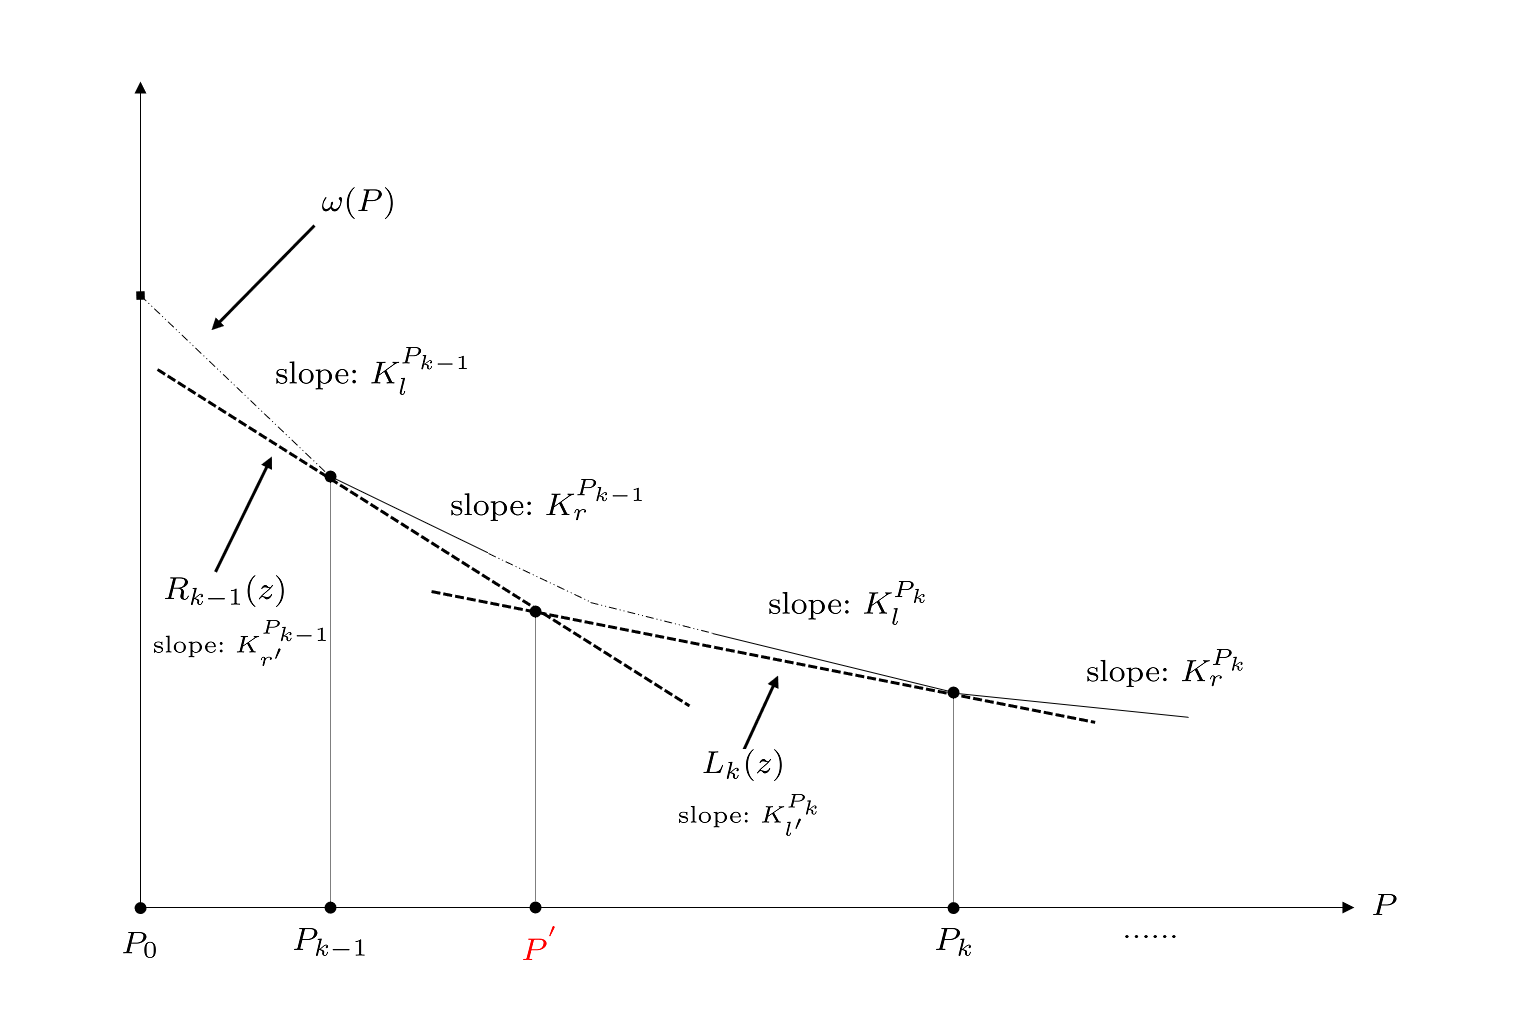
\includegraphics[width=0.9\linewidth]{Figures/IPC}
	\caption{The effects of IPC algorithm applying on the sub-interval.}  %图片的名称
	\label{fig:ImageIPC}   %标签,用作引用
\end{figure}

Then we need to calculate the $\omega(P)$ when given an arbitrary $P$. As stated previously, the value of $\omega(P)$ equals to $\omega_1(P)$. The latter one in fact is a form of simultaneously penalization and subsidization mentioned by Liu et.al.2018.

Then we can follow the basic Cutting Plane(CP) algorithm to solve the tricky exponential inequality constraints $\alpha(s) \leq c_0(s,1)+P$, the specific process are represented in algorithm 2.

\begin{algorithm}[h]\label{algoCP}
\caption{The Cutting Plane(CP) Algorithm to compute $\omega(P)$ for a given $P$.}
\begin{algorithmic}[1]

\begin{description}
  \justifying
  \item[Step 1.] Let $\mathbb{S}'\subseteq \mathbb{S}\setminus \{V\}$ indicates a restricted coalition set, which includes some initial coalitions,
  \vspace{10pt}
  e.g.,$ \{1\},\{2\},\ldots,\{v\}$.
  \item[Step 2.] Find an optimal solution $\bar{\alpha}(\ \cdot \ ,P)$ to LP $\tau(P)$:
  \begin{equation*}
  \max_{\alpha\in \mathbb{R}^v} \big\{ \alpha(V,P): \alpha(s,P) \leq c_0(s,1)+P, \mbox{ for all } s \in \mathbb{S}'\big\}.
  \end{equation*}
  \vspace{-11pt}
  \item[Step 3.]
  Find an optimal solution $s^*$ to the separation problem:
  \begin{equation*}
  \delta = \min \big\{ c_0(s,1)+ P -\bar{\alpha}(s,P): \forall s \in \mathbb{S} \setminus \{V\}\big\}.
  \end{equation*}
  \item[Step 4.]
  If $\delta<0$, then add $s^*$ to $\mathbb{S}'$, and go to step 2; otherwise, return $\omega(P)=c(V,P)-\bar{\alpha}(V,P)$ and the pair of derivatives $(K_{l}^{\bar{\beta}},K_{r}^{\bar{\beta}})$.
\end{description}

\end{algorithmic}
\end{algorithm}

As we all know, the cost arised from the partial players in the grand coalition, that is $c(s,P)$, can be calculated handily by the SPT rule (The corresponding conclusion see Lemma \ref{lem1}).
Now, the question is how to solve the separation problem mentioned above efficiently.

\begin{lem}\label{lem3}
  For the AIPU game, the corresponding separation problem can be sovled in $O(v^2)$ time, which could be shown in the following DP algorithm.
\end{lem}

Assume that the processing jobs satisfy $t_1 \geq t_2 \geq \ldots \geq t_v$. For the separation problem $\delta_{AIPU} = \min \big\{ C'(S,P) -\bar{\alpha}(S,P): \forall S \in \mathbb{S} \setminus \{V\}\big\}$, where $C'(S,P)$ can be obtained by the SPT rule. That means if add a new player $k\notin S$ into $S$, where $|S| =u$, the increment for the restricted separation problem is $(u+1)t_k-\alpha_k$, which will be shown in the recursion in \textbf{Step 3}.

\begin{algorithm}[h]\label{algoDP}
\caption{The Dynamic Programming(DP) Algorithm to Solve the seperation problem.}
\begin{algorithmic}[1]

% the coalition $s$ is a subset of $\{1,2,\ldots,k\}$.

\begin{description}
  \item[Step 1.] Initially, let $D(k,u)$ indicate the minimum objective value of the restricted problem of separation \\
  \vspace{10pt}
  problem $\delta_{AIPU}$, where $k$ is a player in the grand coalition and $u$ is the number of players included in $S$. So $ k \in \{1,2,\ldots,v\}$ and $u\in \{0,1,\ldots,v\}$.

  \item[Step 2.] Given the initial conditions $D(1,0) = P$ and $D(1,1) = t_1 - \beta_1 +P$. The boundary conditions are \\
  \vspace{10pt}
  $D(k,u) = \infty$ if $u > k$, for all $k \in V$.
  \item[Step 3.] Given the recursion:
  \begin{equation*}
  D(k,u)= \min \left\{
  \begin{aligned}
  & D(k-1,u), \text{for the case when} \ s^* \ \text{does not contain} \ k, \\
  & D(k-1,u-1) + u t_k - \alpha_k ,\text{for the case when} \ s^* \ \text{contains} \ k.
  \end{aligned}
  \right.
  \end{equation*}

  \item[Step 4.] Obtain the optimal objective value of separation problem by
  $\delta_{IVPU} = \min\{D(v,u): u\in \{1,2,\ldots,v-1\}\}$.
   return $\delta_{AIPU}$.
\end{description}

\end{algorithmic}
\end{algorithm}

{The DP Algorithm can solve the separation problem $\delta_{AIPU}$ in $O(v^2)$ time.}
Notice that $k \in \{1,2,\ldots,v\}$ and $u\in \{0,1,\ldots,v\}$ for the $D(k,u)$, so the total running time is in $O(v^2)$.
